\documentclass[11pt]{jarticle}

\usepackage[dvipdfmx]{graphicx}
\usepackage{listings}

\lstset{
    basicstyle={\ttfamily\small}, %書体の指定
    frame=tRBl, %フレームの指定
    framesep=10pt, %フレームと中身(コード)の間隔
    breaklines=true, %行が長くなった場合の改行
    linewidth=12cm, %フレームの横幅
    lineskip=-0.5ex, %行間の調整
    tabsize=2 %Tabを何文字幅にするかの指定
}

\setlength{\oddsidemargin}{-6.35mm}
\setlength{\textwidth}{171.9mm}

\begin{document}

\title{画像処理実験 第1回}
\author{09430565\\大橋虎ノ介}
\date{\number\year 年\number\month 月\number\day 日}
\maketitle

\section{[1.1]-[1.3]の画像}


\includegraphics[scale=.5]{./img/download11.png}


\includegraphics[scale=.5]{./img/download12.png}


\includegraphics[scale=.5]{./img/download13.png}

\section{[1.4] javascriptでの実装}

{\bf 赤成分のみの画像}

以下のプログラムを実行し,下のような画像が得られた.

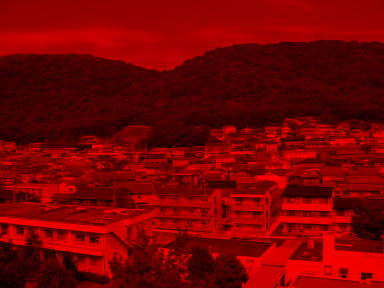
\includegraphics[scale=.5]{./img/js_redonly.png}

\begin{lstlisting}
function process(dst,wdt,hgt, src){
 var y,x,p;
 for(y=0;y<hgt;y++) for(x=0;x<wdt;x++){
   p=(y*wdt+x)*4;
   dst[p+0]=src[p+0];
   dst[p+1]=0;
   dst[p+2]=0;
   dst[p+3]=255;
 }
}
\end{lstlisting}


{\bf 画像の拡大}

以下のプログラムを実行し,下のような画像が得られた.

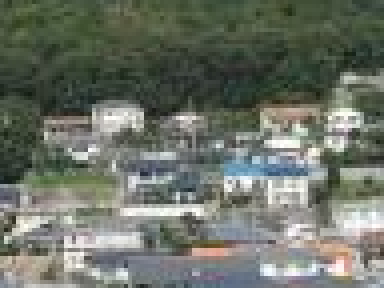
\includegraphics[scale=.5]{./img/js_kakudai.png}

\begin{lstlisting}
function process(dst,wdt,hgt, src){
  var y,x,p,xx,yy;
  for(y=0;y<hgt;y++) for(x=0;x<wdt;x++){
    xx = Math.round(x/4) + 200;
    yy = Math.round(y/4) + 100;
    p=(yy*wdt+xx)*4;
    d=(y*wdt+x)*4;
    dst[d+0]=src[p+0];
    dst[d+1]=src[p+1];
    dst[d+2]=src[p+2];
    dst[d+3]=255;
  }
}
\end{lstlisting}


{\bf 双線形補間}

以下のプログラムを実行し,下のような画像が得られた.

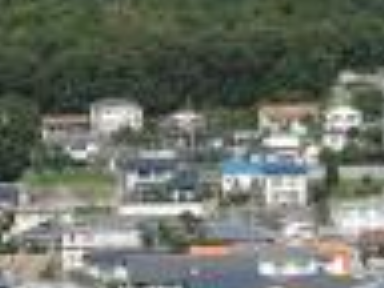
\includegraphics[scale=.5]{./img/js_sousennkei.png}

\begin{lstlisting}
function process(dst,wdt,hgt, src){
  var y,x,p,xx,yy,ix,iy;
  for(y=0;y<hgt;y++) for(x=0;x<wdt;x++){
    xx = x/4 + 200;
    yy = y/4 + 100;
    ix = Math.floor(xx);
    iy = Math.floor(yy);
    xx -= ix;
    yy -= iy;
    p=(iy*wdt+ix)*4;
    d=(y*wdt+x)*4;
    dst[d+0]=(1-yy)*(1-xx)*src[p              +0] +
             (1-yy)*(  xx)*src[p +         4 + 0] +
             (  yy)*(1-xx)*src[p + wdt*4     + 0] +
             (  yy)*(  xx)*src[p + wdt*4 + 4 + 0];
    dst[d+1]=(1-yy)*(1-xx)*src[p              +1] +
             (1-yy)*(  xx)*src[p +         4 + 1] +
             (  yy)*(1-xx)*src[p + wdt*4     + 1] +
             (  yy)*(  xx)*src[p + wdt*4 + 4 + 1];
    dst[d+2]=(1-yy)*(1-xx)*src[p              +2] +
             (1-yy)*(  xx)*src[p +         4 + 2] +
             (  yy)*(1-xx)*src[p + wdt*4     + 2] +
             (  yy)*(  xx)*src[p + wdt*4 + 4 + 2];
    dst[d+3]=255;
  }
}
\end{lstlisting}

\section{[1.5] c言語での実装}

ここでは,javascriptで使用したアルゴリズムをc言語で実装し,スマホで撮影した画像を処理した.
いかに元画像を示す.

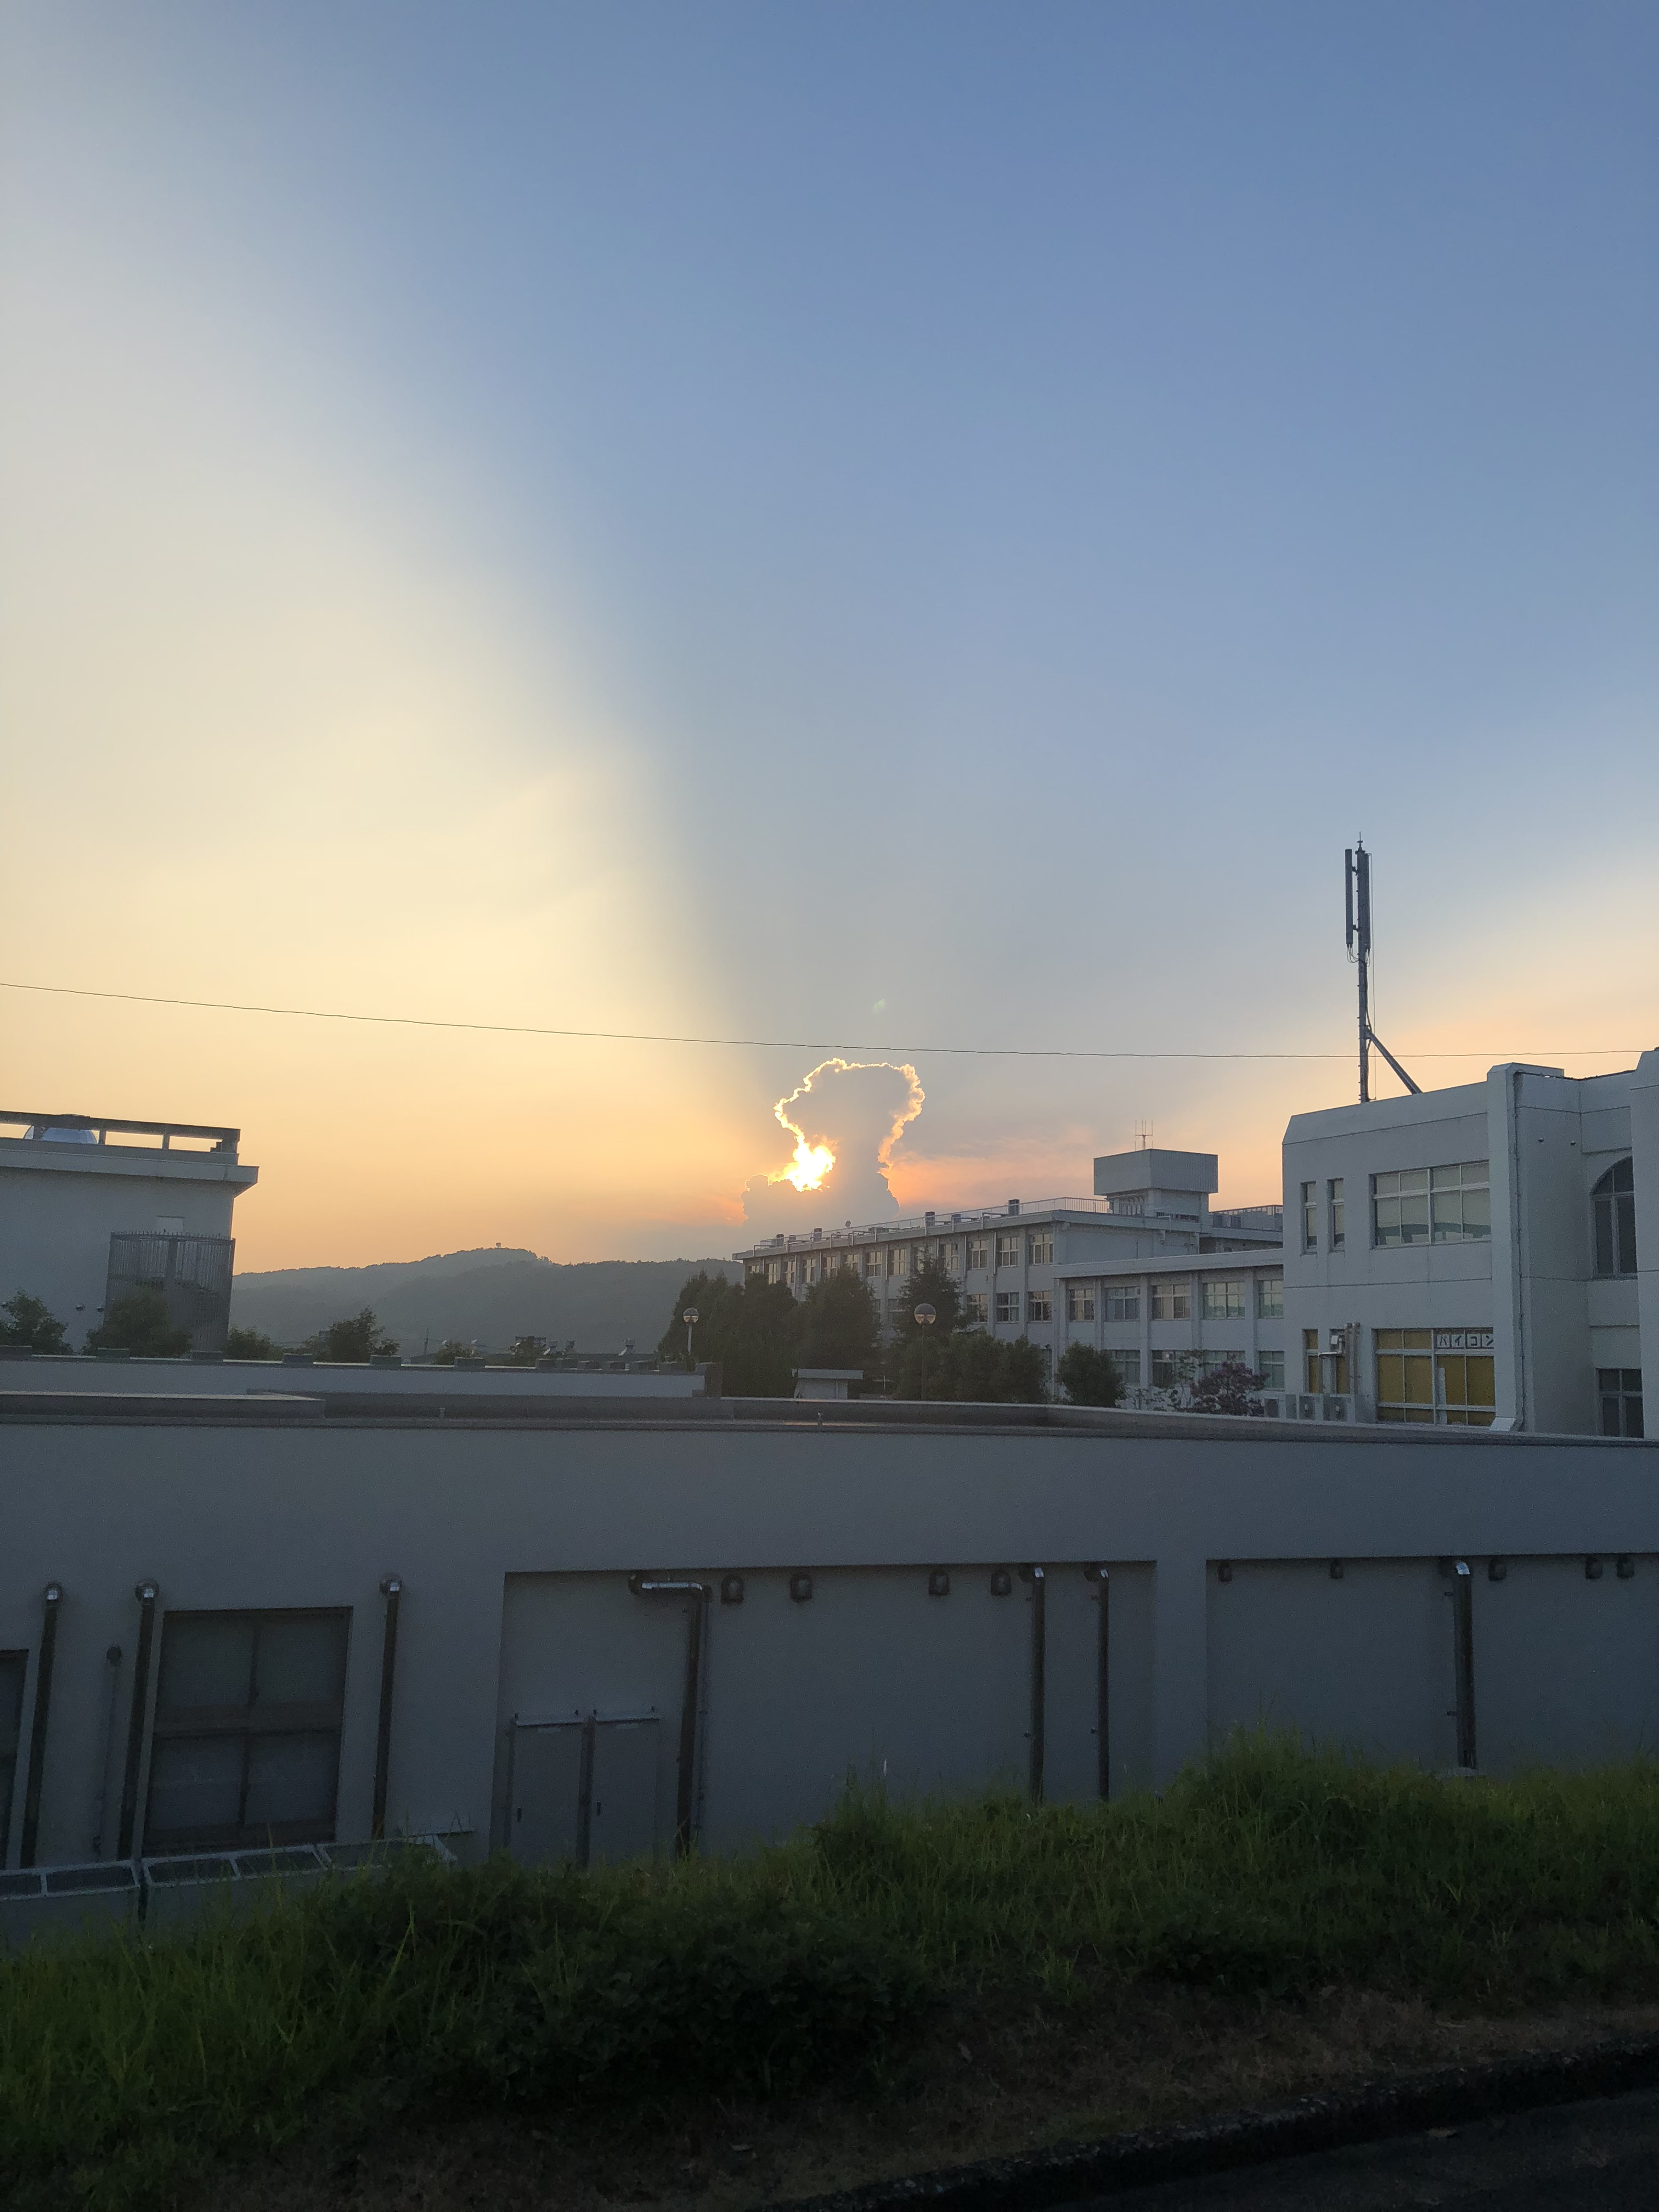
\includegraphics[scale=.1]{./img/tsuyama.jpg}


{\bf 赤成分のみの画像}

以下のプログラムを実行し,下のような画像が得られた.

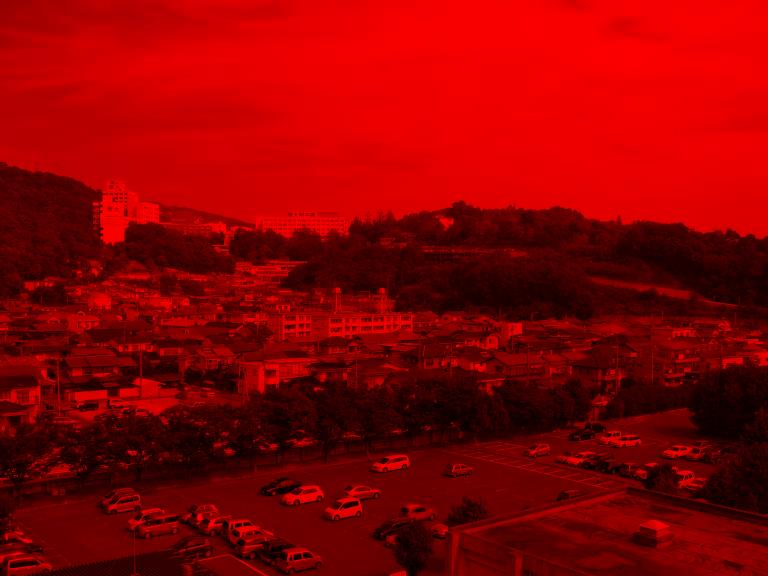
\includegraphics[scale=.5]{./img/red.jpg}

スマホで撮影した画像を処理した.

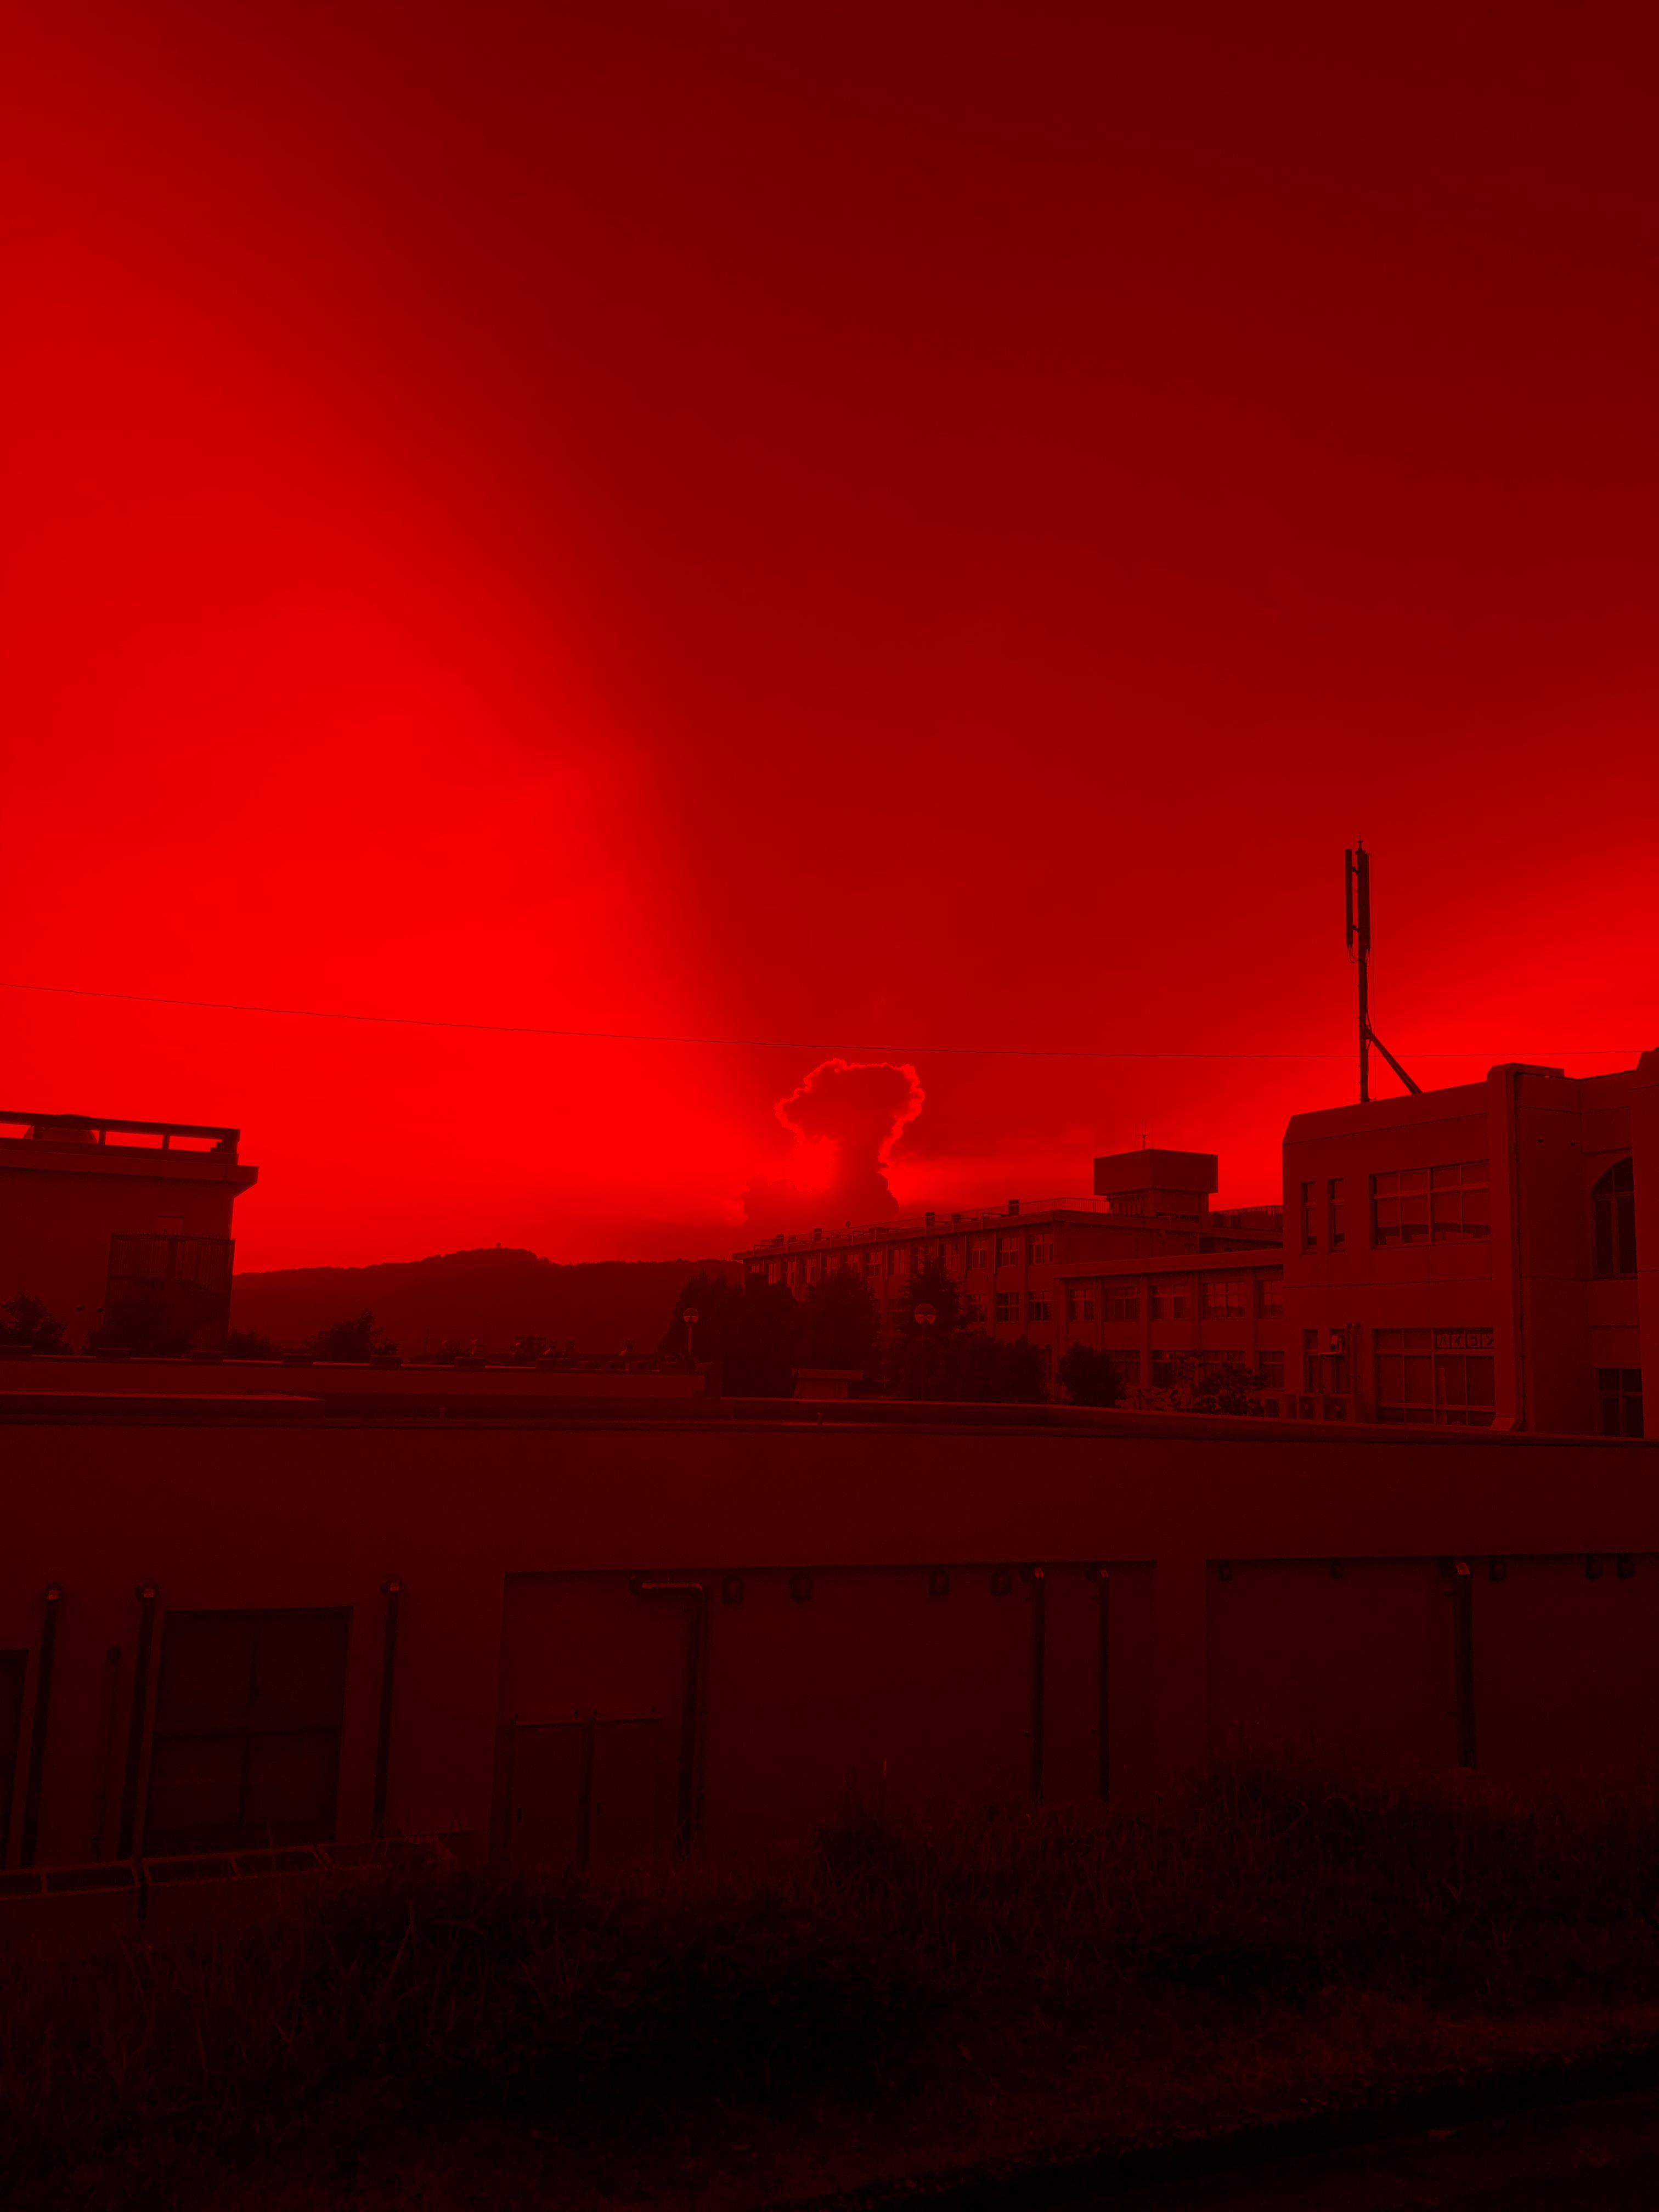
\includegraphics[scale=.1]{./img/tsuyama_red.jpg}

\begin{lstlisting}
void Process(Image*dst,Image*src){
  int x,y;
  for(y=0;y<src->H;y++)
    for(x=0;x<src->W;x++){
      dst->data[(y * dst->W + x) * 3 + 0] = src->data[(y * src->W + x) * 3 + 0];
    }
}
\end{lstlisting}

{\bf 画像の拡大}

以下のプログラムを実行し,下のような画像が得られた.

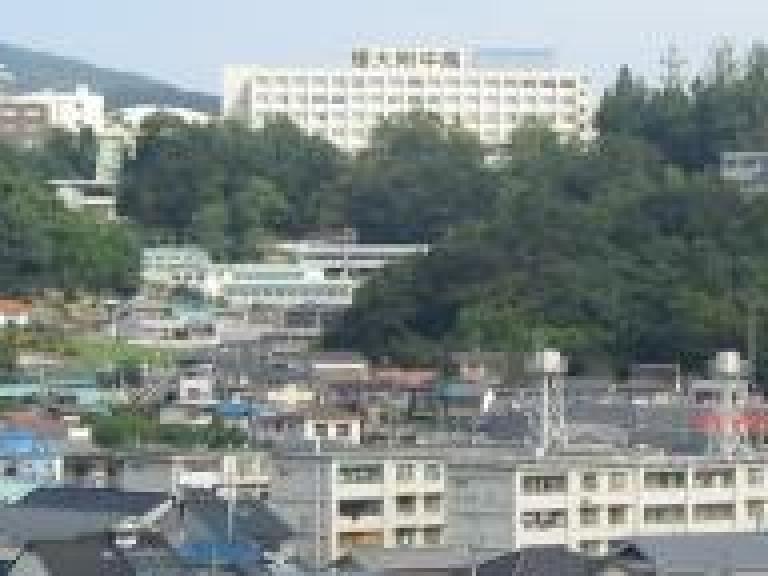
\includegraphics[scale=.5]{./img/kakudai.jpg}

スマホで撮影した画像を処理した.


\includegraphics[scale=.1]{./img/tsuyama_kakudai.jpg}

\begin{lstlisting}
void Process(Image*dst,Image*src){
    int x, y, p, d, xx, yy;
    for(y=0; y<src->H; y++)
        for(x=0; x<src->W; x++){
            xx = x / 4 + 200;
            yy = y / 4 + 200;

            p = (yy * src->W + xx) * 3;
            d = (y * src->W + x) * 3;
       
            dst->data[d + 0] = src->data[p + 0];
            dst->data[d + 1] = src->data[p + 1];
            dst->data[d + 2] = src->data[p + 2];
        }
}
\end{lstlisting}


{\bf 双線形補間}

以下のプログラムを実行し,下のような画像が得られた.

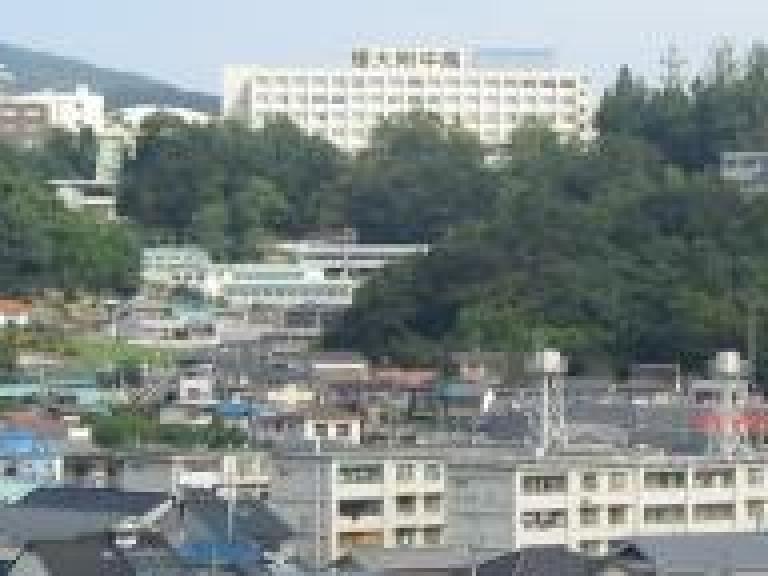
\includegraphics[scale=.5]{./img/sousennkei.jpg}

スマホで撮影した画像を処理した.


\includegraphics[scale=.1]{./img/tsuyama_sousenkei.jpg}

\begin{lstlisting}
void Process(Image*dst,Image*src){
    int x, y, p, d, xx, yy;
    float fx, fy;
    for(y=0; y<src->H; y++)
        for(x=0; x<src->W; x++){
            fx = x / 4 + 200;
            fy = y / 4 + 200;
            xx = fx;
            yy = fy;
            fx -= xx;
            fy -= yy;

            p = (yy * src->W + xx) * 3;
            d = (y * src->W + x) * 3;
     
            dst->data[d + 0] = (1 - fy) * (1 - fx) * src->data[p + 0] +
                (1 - fy) * fx * src->data[p + 4 + 0] +
                fy * (1 - fx) * src->data[p + dst->W * 4 + 0] +
                fy * fx * src->data[p + dst->W * 4 + 4 + 0];
            dst->data[d + 1] = (1 - fy) * (1 - fx) * src->data[p + 1] +
                (1 - fy) * fx * src->data[p + 4 + 1] +
                fy * (1 - fx) * src->data[p + dst->W * 4 + 1] +
                fy * fx * src->data[p + dst->W * 4 + 4 + 1];
            dst->data[d + 2] = (1 - fy) * (1 - fx) * src->data[p + 2] +
                (1 - fy) * fx * src->data[p + 4 + 2] +
                fy * (1 - fx) * src->data[p + dst->W * 4 + 2] +
                fy * fx * src->data[p + dst->W * 4 + 4 + 2];
        }
}
\end{lstlisting}
\section{感想}

まず,環境構築に時間がかかってしまった.
Visual Studioの過去のバージョンのコマンドプロンプトを起動してしまうのか分からないが,コマンドによるコンパイルはできなかった.
VS上でビルドすることで解決した.

latexについて,texlive-lang-japaneseでソースコードを乗せるためにlistingsパッケージを使おうとしたが見つからずはまった.
docker-ubuntu-texlive-jaというdockerイメージを見つけたので,それを使うことで解決した.

実験について,初回ということもあるのか資料が丁寧で分かりやすかった.

\end{document}
